\documentclass[11pt]{article}
\usepackage[margin=1in]{geometry}

\usepackage[utf8]{inputenc}
\usepackage[T1]{fontenc}
\usepackage{polski}
\usepackage{amsmath}
\usepackage{graphicx}

\usepackage{amsfonts}




\edef\restoreparindent{\parindent=\the\parindent\relax}
\usepackage{parskip}
\restoreparindent


\newcommand{\pointsto}[1]{$\rightarrow$ zbiór 2020 {#1}}

\newcounter{exercise}
\newenvironment{exercise}[1]{\refstepcounter{exercise}\par\medskip
   \noindent\textbf{Zadanie~\theexercise.} (#1) \rmfamily}{\medskip}

\begin{document}

\begin{titlepage}
   \begin{center}
       \vspace*{1cm}

       \begin{huge}
       \textbf{Zbiór zadań z egzaminów przedmiotu \\ Języki Formalne i Złożoność Obliczeniowa} \\
        (znanego jako JFIZO)
        \end{huge}

       \vspace{.5cm}
       2006 - 2022
            
       \vspace{1.5cm}

       \textbf{Bartłomiej Grochowski}


       \vspace{2cm}
     
       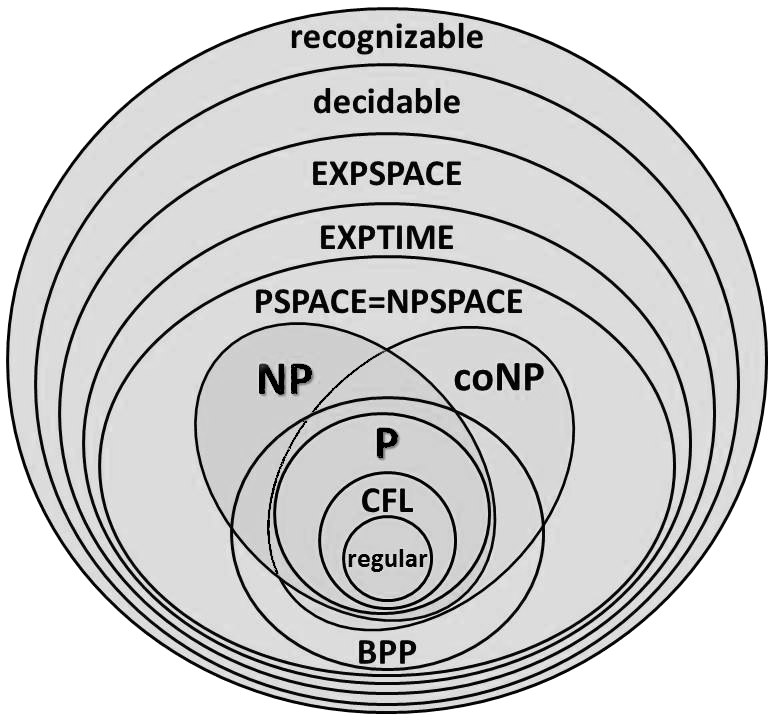
\includegraphics[width=0.4\textwidth]{diagram.png}
            
       \vspace{1cm}
       Treści znalezionych zadań czytelnie zapisane. \\
       Powodzenia...
            
   \end{center}
\end{titlepage}




\section{Części pierwsze}

% JFIZO 2006 cz I
\begin{exercise}{2006 z1}
Czy język $\{a^ib^jc^kd^l \in \{a,b,c,d\}^* : l=0 \lor i=j=k\}$ jest bezkontekstowy?
\end{exercise}

\begin{exercise}{2006 z2}
\pointsto{z17}
\end{exercise}

\begin{exercise}{2006 z3}
\pointsto{z18, z19}
\end{exercise}

% JFIZO 2006P cz I
\begin{exercise}{2006P/1}
Niech L będzie językiem tych słów $w \in \{a,b,c\}^*$, dla których żadne dwie z liczb $|w|_a, |w|_b, |w|_c$ nie są względnie pierwsze. Czy $L$ jest językiem bezkontekstowym?
\end{exercise}

\begin{exercise}{2006P/2}
Rozważmy alfabet $\Sigma$ składający się z czterech symboli: red a, red b, blue a, blue b. Ile co najmniej stanów musi mieć DFA rozpoznający
\begin{itemize}
    \item[a)] (łatwe) $L = \{ w \in \Sigma^* :$ 10 od końca 'a' jest 'blue' $\}$
    \item[b)] (trudne) $L = \{ w \in \Sigma^* :$ 10 od końca 'a' jest 'blue' i jednocz. 10 od końca 'blue' symbolem $\}$
\end{itemize}
\end{exercise}

\begin{exercise}{2006P/3}
Udowodnij, że język tych słów nad alfabetem $\{a,b,c\}$, które zaczynają się od niepustego palindromu parzystej długości, nie jest regularny.
\end{exercise}

% JFIZO 2007 cz I
\begin{exercise}{2007/1}
Niech $L \subseteq \{0,1\}^*$ będzie językiem regularnym.
\begin{itemize}
    \item $2L = \{wv \in \{0,1\}^* : |w| = |v| \land w \in L\}$
    \item $L_2 = \{wv \in \{0,1\}^* : |w| = |v| \land \exists z \in L.\ |z| = |w|\}$
\end{itemize}
\begin{itemize}
    \item[a)] Czy $2L$ jest regularny?
    \item[b)] Czy $L_2$ jest regularny?
\end{itemize}
\end{exercise}

% JFIZO 2007P cz I
\begin{exercise}{2007P/1}
\pointsto{z63}
\end{exercise}

\begin{exercise}{2007P/2}
Niech $L_3$ oznacza język poprawnie rozstawionych nawiasów trzech rodzajów, bez zagnieżdżenia w nawiasach tego samego typu. Np. do $L_3$ nie może należeć żadne słowo postaci x\{y\{z\}t\}u, gdzie w słowie 'y' nie występuje '\}' ( '\{' - którykolwiek z trzech rodzajów nawiasów). Napisz regex oznaczający język $L_3$. Wyrażenie może mieć max 35 wystąpień nawiasów.
\end{exercise}

\begin{exercise}{2007P/3}
Niech $L_n$ będzie językiem poprawnie rozstawionych nawiasów n rodzajów, bez zagnieżdżania w nawiasach tego samego typu, analogicznie jak w poprzednim zadaniu. Ile stanów ma najmniejszy DFA rozpoznający $L_n$?
\end{exercise}

% JFIZO 2008 cz I
\begin{exercise}{2008/1}
\pointsto{z26}
\end{exercise}

\begin{exercise}{2008/2}
\pointsto{z48}
\end{exercise}

\begin{exercise}{2008/3}
\pointsto{z54}
\end{exercise}

% JFIZO 2008P cz I
\begin{exercise}{2008P/1}
Czy język składający się z tych słów $w$ nad alfabetem $\{a,b,c\}$, które zaczynają się od palindromu parzystej długości i dłuższego niż połowa długości $w$, jest bezkontekstowy?
\end{exercise}


% JFIZO 2009 cz I
\begin{exercise}{2009/1}
\pointsto{z27}
\end{exercise}
\begin{exercise}{2009/2}
\pointsto{z28}
\end{exercise}
\begin{exercise}{2009/3}
Rozważmy język $L = \{ w \in \{0,1\}^* : |w|_0 = |w|_1 \}$.
\begin{itemize}
    \item[a)] Podaj CFG G w postaci normalnej Greibach t.że $L = L_G$
    \item[b)] Podaj CFG G w postaci normalnej Chomsky'ego t.że $L = L_G$
    \item[c)] Wyjaśnij, po co potrzebujemy twierdzenia o postaci normalnej Greibach.
    \item[d)] Wyjaśnij, po co potrzebujemy twierdzenia o postaci normalnej Chomsky'ego.
\end{itemize}
\end{exercise}

% JFIZO 2009P cz I
\begin{exercise}{2009P/1}
Niech $L(L_1,L_2,L_3) = \{xyz \in \{0,1\}^* : x \in L_1, y \in L_2, z \in L_3, |x| = |y| = |z|\}$. Czy $L(L_1,L_2,L_3)$ jest CFL jeśli:
\begin{itemize}
    \item[a)] $L_1 = L_3 = L_{0^*}$, zaś $L_2 = L_{0*10*10*}$ ?
    \item[b)] $L_1 = L_2 = L_{0^*}$, zaś $L_3 = L_{0*10*10*}$ ?
\end{itemize}
\end{exercise}

\begin{exercise}{2009P/2}
\pointsto{z30}
\end{exercise}

\begin{exercise}{2009P/3}
\pointsto{z31}
\end{exercise}

% JFIZO 2010 cz I
\begin{exercise}{2010/1}
\pointsto{z29}
\end{exercise}

\begin{exercise}{2010/2}
\pointsto{z55}
\end{exercise}

\begin{exercise}{2010/3}
\pointsto{z62}
\end{exercise}

% JFIZO 2011 cz I
\bigskip
Stefanką ze słów $w,v_1,...,v_l$ nazywamy słowo postaci $w_0v_1w_1...w_{l-1}v_lw_l$, gdzie $w = w_0w_1...w_l$.  Stefanką z języków $L_1,L_2$ nazwiemy zbiór wszystkich słów $w'$, dla których istnieją $l \in \mathbb{N}$ i słowa $w \in L_1$ i $v_1,v_2,...,v_l \in L_2$, t.że $w'$ jest stefanką z $w,v_1,...,v_l$

\begin{exercise}{2011/1}
Niech $L_1, L_2$ języki regularne, t.że istnieją NDFA $A_1, A_2$ mające odpowiednio $n_1, n_2$ stanów, rozpoznające odpowiednio języki $L_1, L_2$.
\begin{itemize}
    \item[a)] Udowodnij, że $L=Stefanka(L_1,L_2)$ daje się rozpoznawać NDFA o $O(n_1n_2)$ stanach.
    \item[b)]  Udowodnij, że oszacowania $O(n_1n_2)$ na liczbę stanów automatu niedeterministycznego rozpoznającego $L$ nie da się poprawić.
\end{itemize}
\noindent \textit{Wskazówka: Wystarczy, że języki $L_1 \subseteq 0^*$ i $L_2 \subseteq 1^*$ będą odpowiednio dobranymi językami jednoelementowymi.}
\end{exercise}

\begin{exercise}{2011/2}
(trudne) Załóżmy, że $L_1, L_2$ są językami regularnymi, t.że istnieją DFA $A_1,A_2$ mające odpowiednio $n_1,n_2$ stanów. Czy wynika z tego, że istnieje DFA o $O(n_1n_2)$ stanach rozpoznający język $L=Stefanka(L_1,L_2)$? \\
\textit{Wskazówka: W rozwiązaniu $n_2 = 3$, a rozpoznanie $L$ wymaga rzędu $n_1^2$ stanów}
\end{exercise}

\begin{exercise}{2011/3}
Czy stefanka z dwóch języków bezkontekstowych zawsze jest językiem bezkontekstowym?
\end{exercise}

% JFIZO 2013 cz I
\begin{exercise}{2013/1}
\pointsto{z35}
\end{exercise}

\begin{exercise}{2013/2}
\pointsto{z36}
\end{exercise}

\begin{exercise}{2013/3}
\pointsto{z37}
\end{exercise}

% JFIZO 2013P cz I
\begin{exercise}{2013P/1}
\pointsto{z8}
\end{exercise}

\begin{exercise}{2013P/2}
\pointsto{z9}
\end{exercise}

\begin{exercise}{2013P/3}
\pointsto{z10}
\end{exercise}

% JFIZO 2014 cz I
\begin{exercise}{2014/1}
\pointsto{z38}
\end{exercise}

\begin{exercise}{2014/2}
\pointsto{z39}
\end{exercise}

\begin{exercise}{2014/3}
\pointsto{z40}
\end{exercise}

% JFIZO 2014P cz I
\begin{exercise}{2014P/1}
Jaki jest indeks języka składającego się ze wszystkich słów $w$ nad alfabetem $\{0,1\}$, takich że wśród dziewięciu ostatnich symboli słowa $0^9w$ jest parzyście wiele jedynek?
\end{exercise}

\begin{exercise}{2014P/2}
Niech $f: \{0,1\}^9 \rightarrow \{0,1\}$ będzie dowolną funkcją i niech $L_f$ będzie językiem składającym się ze wszystkich słów $w$ nad alfabetem $\{0,1\}$, takich że $f(v)=1$, gdzie $v$ to słowo składające się z dziewięciu ostatnich symboli słowa $0^9w$. Rozważmy dwa warunki:
\begin{itemize}
    \item[I.] funkcja $f$ zależy od pierwszego argumentu, tzn $\exists v \in \{0,1\}^8$ t.że $f(0v) \neq f(1v)$
    \item[II.] indeks $L_f = 512$
\end{itemize}
\begin{itemize}
    \item[a)] Czy $I \Rightarrow II$ ?
    \item[b)] Czy $II \Rightarrow I$ ?
\end{itemize}

\end{exercise}

\begin{exercise}{2014P/3}
Czy język $L$ składający się z tych słów, które są binarnymi zapisami liczb~$3^{2^n}$, dla wszystkich liczb naturalnych $n$, jest bezkontekstowy?
\end{exercise}

% JFIZO 2016 cz I
\bigskip
Przez $CFL_i$ będziemy oznaczać te języki bezkontekstowe, dla któyrch istnieje gramatyka mająca, oprócz symbolu początkowego $S$, który nie może pojawić się po prawej stronie żadnej reguły, co najwyżej $i$ nieterminali.

Przez $R_i$ będziemy oznaczać język oznaczany przez wyrażenie regularne $a_ia_i^*$ nad alfabetem $\{a_i\}$. Niech $L_0 = \{ \epsilon \}$ i niech $L_{i+1} = L_iR_{i+1}$.
\begin{exercise}{2016/1}
\begin{itemize}
    \item[a)] Jakie jest najmniejsze $i$ dla którego język oznaczany przez wyrażenie regularne $(0^*10^*10^*)^*$ należy do $CFL_i$?
    \item[b)] Jakie jest najmniejsze $i$ dla którego język składający się z tych słów nad $\{0,1\}$ w których jest nieparzyście wiele jedynek i nieparzyście wiele zer należy do $CFL_i$?
\end{itemize}
\end{exercise}

\begin{exercise}{2016/2}
\begin{itemize}
    \item[a)] Udowodnij następujący Lemat o Pompowaniu dla $CFL_1$: Dla każdego języka $L\in CFL_1$ istnieje stała $k$ taka że dla każdego słowa $w \in L$ o długości większej od $k$ istnieje podział $v_0s_1v_1s_2...s_lv_l$ słowa $w$, i podział $x_iy_iz_i$ każdego ze słów $s_i$ takie że:
    \begin{itemize}
        \item $l \leq k$
        \item każde $v_i$ i każde $y_i$ ma długość co najwyżej $k$
        \item dla każdych $1 \leq i,j \leq l$ słowo $v_0s_1v_1s_2...v_{i-1}x_is_jz_iv_i...s_lv_l$ powstałe ze słowa $w$ przez zastąpienie wystąpienia fragmentu $y_i$ słowa $s_i$ w $w$ przez $s_j$, również należy do $L$.
    \end{itemize}
    \item[b)] Użyj powyższego Lematu o Pompowaniu aby pokazać, że $L_3 \notin CFL_1$.
\end{itemize}
\end{exercise}

\begin{exercise}{2016/3}
Niech $n \in \mathbb{N}$. Jakie jest najmniejsze $k$ dla którego $L_{2n} \in CFL_k$?
\end{exercise}

% JFIZO 2016P cz I
\begin{exercise}{2016P/1}
\pointsto{z78, z79}
\end{exercise}

\begin{exercise}{2016P/2}
\pointsto{z80}
\end{exercise}

\begin{exercise}{2016P/3}
\pointsto{z81}
\end{exercise}


% JFIZO 2019 cz I
\begin{exercise}{2019/1}
\pointsto{z11}
\end{exercise}

\begin{exercise}{2019/2}
\pointsto{z12}
\end{exercise}

\begin{exercise}{2019/3}
\pointsto{z56}
\end{exercise}

% JFIZO 2020 cz I
\begin{exercise}{2020/1}
Pokaż, że istnieje NFA $A$, t. że ma $<$ 20 stanów i każde słowo nad $\Sigma$ mające długość $\leq$ 100 należy do $L_A$, ale $L_A \neq \Sigma^*$
\end{exercise}

\begin{exercise}{2020/2}
Niech $L \subseteq \{a,b\}^*$ będzie językiem regularnym dającym się rozstrzygać DFA o $n$ stanach. Pokaż, że język $L' = \{w \in \{a,b\}^* : \exists v.\ |v| = k*|w| \land wv \in L\}$, daje się rozstrzygać DFA o wykładniczej względem $n$ liczbie stanów.
\end{exercise}

\begin{exercise}{2020/3}
Dla danego języka $L \subseteq \{a,b,c\}^*$ niech $L_{(2)} = \{wv \in \{a,b,c\}^*\ : \ |v| = |w| \land w \in L\}$. Czy z tego, że $L$ jest CFL wynika że $L_{(2)}$ jest CFL?
\end{exercise}

% JFIZO 2021 cz I
\begin{exercise}{2021/1}
Język $L_{v \neq w} = \{ vw : v,w \in \{0,1\}^*, |v| = |w|, v \neq w \}$ jest bezkontekstowy, zatem daje się go rozstrzygać jakimś NPDA. Pokaż, że języka $L_{v \neq w}$ nie da się rozstrzygać deterministycznym automatem z jednym licznikiem.
\end{exercise}

\bigskip
W kolejnych dwóch zadaniach rozważamy Odrobinkę Niedeterministyczne Automaty Skończone (ONFA). Taki automat to krotka $\langle \Sigma, Q, Q_0, F, \delta \rangle$, gdzie $Q_0 \subseteq Q$ jest zbiorem dopuszczalnych stanów początkowych. Słowo $w$ jest akceptowane przez taki automat gdy istnieje $q_0 \in Q_0$ takie że $\hat{\delta}(q_0,w)~\in~F$.

\begin{exercise}{2021/2}
Pokaż, że istnieje ciąg języków $\{L_i\}_{i\in\mathbb{N}}$ i stałe $c,k > 0$ takie, że każdy $L_i$ daje się rozstrzygać przy pomocy ONFA o nie więcej niż $ki$ stanach, ale żaden $L_i$ nie daje się rozstrzygać przy pomocy DFA o mniej niż $2^{ci}$ stanach.
\end{exercise}

\begin{exercise}{2021/3}
Pokaż, że istnieje ciąg języków $\{L_i\}_{i\in\mathbb{N}}$ i stałe $c,k > 0$ takie, że każdy $L_i$ daje się rozstrzygać przy pomocy NFA o nie więcej niż $ki$ stanach, ale żaden $L_i$ nie daje się rozstrzygać przy pomocy ONFA o mniej niż $2^{ci}$ stanach.
\end{exercise}

% JFIZO 2021 cz I
\bigskip
W trzech kolejnych zadaniach umawiamy się, że skończony alfabet $\Sigma$ nie zawiera symbolu $\#$. Dla danego języka $L \subseteq \Sigma^*$ definiujemy $L_\# = \{w\#v : vw \in L\}$.
\begin{exercise}{2021P/1}
Załóżmy że $L$ jest językiem regularnym dającym się rozstrzygać pewnym DFA o $n$ stanach. Pokaż że w takim razie $L_\#$ daje się rozstrzygać pewnym DFA o $cn^n$, dla pewnej stałej $c$ niezależnej od $L$.
\end{exercise}

\begin{exercise}{2021P/2}
Pokaż, że szacowania z poprzedniego zadania nie da się poprawić, to znaczy, że dla każdego (dostatecznie dużego) $n \in \mathbb{N}$ istnieje język $L \subseteq \Sigma^*$ dający się rozstrzygać DFA o $n$ stanach i taki, że każdy DFA rozstrzygający $L_\#$ ma przynajmniej $n^n$ stanów.
\end{exercise}

\begin{exercise}{2021P/3}
\begin{itemize}
    \item[a)] (trudne) Pokaż, że dla każdego języka bezkontekstowego $L$, język $L_\#$ jest również bezkontekstowy.
    \item[b)] Niech $L$ będzie językiem dobrze rozstawionych nawiasów. Pokaż, że język $L_\#$ jest bezkontekstowy.
\end{itemize}
\end{exercise}

% JFIZO 2022 cz I
\begin{exercise}{2022/1}
Udowodnij, że język $\{ a^nb^nc^m : n \neq m\}$ nie jest CFL. \\
\textit{Wskazówka: Lemat o pompowaniu wydaje się nie działać. A gdyby w sformułowaniu lematu zastąpić wszystkie wystąpienia symbolu $|\_|$ (oznaczającego długość słowa) symbolem $|\_|_c$ (oznaczającym liczbę wystąpień literki c)?}
\end{exercise}

\bigskip
W kolejnych dwóch zadaniach dla automatu A, przez $L_A^{1}$ oznaczymy zbiór takich słów $w$, dla których istnieje dokładnie jedna ścieżka w A, prowadząca od stanu początkowego do jakiegoś stanu akceptującego, taka że ciąg etykiet krawędzi na tej ścieżce tworzy słowo $w$.

\begin{exercise}{2022/2}
Pokaż, że dla każdego niedeterministycznego automatu skończonego A, język $L_A^{1}$ jest regularny.
\end{exercise}

\begin{exercise}{2022/3}
Czy istnieje wielomian $p$ taki że dla każdego $n \in \mathbb{N}$ i każdego niedeterministycznego automatu skończonego A o $n$ stanach istnieje niedeterministyczny automat skończony B, o co najwyżej $p(n)$ stanach, taki że $L_A^{1} = L_B$?
\end{exercise}



\newpage
\section{Części drugie}

% JFIZO 2006 cz II
\begin{exercise}{2006/4}
Dla całkowitej funkcji rekurencyjnej $f$ definiujemy:
\begin{itemize}
    \item $h^f(n) = max\{k:f(k) = n\},$
    \item $h_f(n) = min \{k:f(k) = n\}$
\end{itemize}
(minimum i maksimum ze zbioru pustego są nieokreślone, podobnie jak maksimum ze zbioru nieskończonego). Które z funkcji $h^f, h_f$ są rekurencyjne (być może częściowe)? Które są całkowite rekurencyjne? Jak zmieni się odpowiedź, jeśli założymy, że $f$ jest 'na'?
\end{exercise}

% JFIZO 2006P cz II
\begin{exercise}{2006P/4}
Niech $W_n$ oznacza dziedzinę funkcji rekurencyjnej obliczanej przez maszynę o numerze $n$. Niech $A \subseteq \mathbb{N}$ będzie rekurencyjnie przeliczalny. Czy wynika z tego, że $\bigcup_{n \in A} W_n$ jest rekurencyjnie przeliczalny?
\end{exercise}

\begin{exercise}{2006P/6}
Funkcję (częściową) $f: \mathbb{N} \rightarrow \mathbb{N}$ nazwiemy 'z grubsza różnowartościową', jeśli każdą wartość przyjmuje ona tylko dla skończonego zbioru argumentów. Czy zbiór wszystkich numerów maszyn obliczających funkcje z grubsza różnowartościowe jest r.e.? Czy jego dopełnienie jest r.e.?
\end{exercise}

% JFIZO 2007 cz II
\begin{exercise}{2007/4}
\pointsto{z110, z111}
\end{exercise}

\begin{exercise}{2007/5}
Niech $L \subset \mathbb{N}$ będzie zbiorem numerów tych programów, które zatrzymują się dla jakiejś liczby parzystej lub nie zatrzymują się dla jakiejś liczby nieparzystej.
\begin{itemize}
    \item[a.] Udowodnij, że ani $L$ ani jego dopełnienie nie są rekurencyjnie przeliczalne.
    \item[b.] Nie powołując się na tw. Rice'a udowodnij, że $L$ nie jest rekurencyjny.
\end{itemize}
\end{exercise}

\begin{exercise}{2007/6}
\pointsto{z98}
\end{exercise}

% JFIZO 2007P cz II
\begin{exercise}{2007P/4}
Niech $A$ będzie zbiorem takich par numerów programów $\langle n,m\rangle$, że dla każdej liczby naturalnej $k$ albo program o numerze $n$ uruchomiony dla danej $k$ się zatrzymuje, a program o numerze $m$ uruchomiony dla danej $k$ się nie zatrzymuje, albo na odwrót. Czy $A$ jest r.e.?
\end{exercise}

\bigskip
Automat chodzący po pierwszej ćwiartce będzie opisany przez skończony zbiór instrukcji będący podzbiorem $Q\times K\times \{T,F\} \times \{T,F\}\times Q \times \{n,s,e,w\}$, gdzie Q jest skończonym zbiorem stanów, K skończonym zbiorem kolorów i będący funkcją (częściową) ze względu na cztery pierwsze argumenty. Wejściem automatu jest ćwiartka płaszczyzny: nieskończona, w kierunku wschodnim i północnym, szachownica, której każde pole pokolorowane jest jednym z kolorów ze zbioru K. Na początku swojego działania automat umieszczany jest w (jednym) rogu szachownicy, a następnie w każdym ruchu, w zależności od tego, w jakim jest stanie, na polu jakiego koloru stoi oraz czy jest prawdą, że stoi na zachodnim skraju szachownicy i czy jest prawdą, że stoi na południowym skraju szachownicy, zmienia stan i przechodzi o jedno pole na północ, południe, wschód lub zachód. Instrukcje są tak zbudowane, że nie może opuścić szachownicy. Jeśli automat nie ma instrukcji mówiącej mu jak się ma zachować to zatrzymuje się i akceptuje wejście. Automat jest totalny jeśli akceptuje każde wejście.

\begin{exercise}{2007P/5}
Udowodnij, że problem totalności jest dla automatów chodzących po pierwszej ćwiartce nierozstrzygalny. Gdybyś przy okazji dowodu konstruował jakiś automat, należy opisać ideę jego działania.
\end{exercise}

\begin{exercise}{2007P/6}
(trudne) Czy problem totalności pozostanie nierozstrzygalny, jeśli ograniczymy się do automatów, w których instrukcjach występują tylko litery $w,e$, zaś nie występują litery $n,s$, to znaczy takich, które nigdy nie opuszczają południowego skraju szachownicy? \\
\textit{Komentarz: ciekawe, że problem totalności dla analogicznego automatu chodzącego po dwóch ćwiartkach wydaje się być rozstrzygalny}
\end{exercise}


% JFIZO 2008 cz II

\begin{exercise}{2008/4}
Czy istnieje algorytm rozstrzygający dla danych dwóch deterministycznych PDA, czy istnieje niepuste słowo, które zostanie zaakceptowane przez oba te automaty?
\end{exercise}

\begin{exercise}{2008/5}
Niech $A \subseteq \mathbb{N}$ będzie zbiorem tych liczb naturalnych, które są numerami programów zatrzymujących się dla wszystkich danych. Niech $E \subseteq \mathbb{N}$ będzie zbiorem tych liczb naturalnych, które są numerami programów nie zatrzymujących się dla żadnych danych. Udowodnij, że $E \leq_{rek} A$.
\end{exercise}

\begin{exercise}{2008/6}
Niech $A$ i $E$ będą takie, jak w poprzednim zadaniu. Czy zachodzi nierówność $A \leq_{rek} E$? \\
\textit{Wskazówka: Co było mówione na ćwiczeniach na temat $K \leq_{rek} \overline{K}$?}
\end{exercise}

% JFIZO 2008P cz II
\begin{exercise}{2008P/4}
Funkcja $f:\mathbb{N} \rightarrow \mathbb{N}$ jest całkowita rekurencyjna i taka, że istnieje tylko skończenie wiele liczb naturalnych $n$, dla których $f(n) > f(n+1)$. Czy wynika z tego, że zbiór $f(\mathbb{N})$ jest rekurencyjny?
\end{exercise}

\bigskip
Niech $S \subseteq Z \times Z$ będzie pewnym podzbiorem zbioru punktów kratowych płaszczyzny, t.że $[0,0]\in S$. Przez T oznaczmy zbiór $\{-1,0,1\}$. Dla punktu $[a,b]\in S$ niech $s([a,b])=\{[x,y] \in T^2 : [a+x,b+y]\in S\}$ (oczywiście zawsze zachodzi $[0,0] \in s[a,b]$, zaś $s[a,b]$ można rozumieć jako "zbiór kierunków w jakich można zrobić krok z $[a,b]$ pozostając w zbiorze $S$").

W kolejnych dwóch zadaniach rozpatrujemy automaty skończone spacerujące po zbiorze S. Automat taki dany jest przez skończony zbiór stanów $Q$, ze stanem początkowym $q_0 \in Q$, oraz przez zbiór instrukcji $\pi$, będący funkcją o dziedzinie zawartej w $Q \times \mathcal{P}(T^2)$ i o zbiorze wartości zawartym w $Q \times T^2$ taką, że (*) jeśli $\pi(q,W) = [q',w]$, to $w \in W$.

Jeśli teraz automat znajduje się w stanie $q$ w punkcie $[a,b]\in S$ i jeśli $\pi(q,s([a,b])) = [q',[x,y]]$ to w kolejnym kroku przechodzi do stanu $q'$ i do punktu [a+x,b+y]. Potocznie mówiąc: automat "wie" w jakim jest stanie, i które z ośmiu sąsiednich punktów należą do S, i w zależności od tej swojej wiedzy zmienia stan i przechodzi do jednego z sąsiednich punktów. Zwróć uwagę, że z (*) wynika, że automat nigdy nie opuści zbioru S.

Jeśli automat znajduje się w stanie $q$ w punkcie $[a,b]\in S$ i jeśli $\pi(q,s([a,b]))$ nie jest określone, to automat się zatrzymuje.

Dla ustalonego zbioru S przez problem stopu dla automatów skończonych spacerujących po S rozumiemy problem ustalenia, dla danego $Q,q_0,\pi$, czy opisany powyżej automat uruchomiony w stanie $q_0$ w punkcie $[0,0]$, kiedykolwiek się zatrzyma.

\begin{exercise}{2008P/5}
\begin{itemize}
    \item[a)] Czy problem stopu dla automatów skończonych spacerujących po S jest rozstrzygalny, jeśli $S = \{[a,b] : a,b \geq 0 \}$?
    \item[b)] Czy odpowiedź na pytanie z punktu a) zmieni się jeśli przyjmiemy $S = \{[a,b] : b \geq 0, a\geq -b\}$?
\end{itemize}

\end{exercise}
\begin{exercise}{2008P/6}
Czy problem stopu dla automatów skończonych spacerujących po S jest rozstrzygalny, jeśli $S = \{[a,b] : b \geq 0\}$?
\end{exercise}

% JFIZO 2009 cz II
\bigskip
Przez automat z $k$ rosnącymi licznikami będziemy w kolejnych dwóch zadaniach rozumieć deterministyczny automat, który:

- ma skończony zbiór stanów $Q$ zawierający m. in. $q_0$ i $q_F$
- nie czyta (nie ma) słowa wejściowego
- ma $k$ liczników, to znaczy stosów z jednym symbolem stosowym (różnym niż symbol dna stosu)

i którego wszystkie instrukcje mają format $\langle q,a_1^2,a_1^3,...,a_1^k,a_2^3,...,a_{k-1}^k;q',b^1,...,b^k\rangle$ gdzie $a_i^j$ to albo zdanie \textit{"zawartość licznika i jest nie mniejsza niż zawartość licznika j"} albo jego negacja, zaś każde z $b^i$ jest dodatnią liczbą naturalną.

Instrukcja $\langle q,a_1^2,a_1^3,...,a_1^k,a_2^3,...,a_{k-1}^k;q',b^1,...,b^k\rangle$ może być wykonywana w konfiguracji automatu, w której jest on w stanie $q$, zaś liczby $j_1,j_2,...,j_k$ będące aktualnymi stanami liczników automatu, spełniają warunki $a_1^2,a_1^3,...,a_1^k,a_2^3,...,a_{k-1}^k$. Wynikiem wykonania instrukcji jest wtedy zmiana stanu na $q'$ i zwiększenie j-tego licznika o $b^j$ dla każdego j. Mówiąc po ludzku oznacza to, że automat wie w jakim jest stanie, umie porównać ze sobą liczby na swoich $k$ licznikach i w zależności od tej swojej wiedzy decyduje do jakiego stanu ma przejść i o ile ma zwiększyć zawartości liczników.

Problem stopu dla automatów z k rosnącymi licznikami to, jak łatwo zgadnąć, problem czy dany taki automat, uruchomiony w stanie początkowym $q_0$, ze wszystkimi licznikami równymi zero, kiedykolwiek osiągnie stan końcowy $q_F$.

\begin{exercise}{2009/5}
Czy problem stopu dla automatów z dwoma rosnącymi licznikami jest rozstrzygalny?
\end{exercise}

\begin{exercise}{2009/6}
Czy problem stopu dla automatów z trzema rosnącymi licznikami jest rozstrzygalny?
\end{exercise}

% JFIZO 2009P cz II
\begin{exercise}{2009P/4}
Powiemy, że $A \subseteq \mathbb{N}$ zawiera 'długi odcinek', jeśli istnieje taka liczba naturalna $k$, że wszystkie liczby naturalne z odcinka $[k,2k]$ należą do $A$. Czy zbiór $X$ numerów tych programów (funkcji częściowych), których dziedzina, będąca podzbiorem zbioru liczb naturalnych, zawiera długi odcinek, jest rekurencyjnie przeliczalny?
\end{exercise}

\bigskip
Rozważamy płaszczyznę, po której biega $k$ psów. Startują one jednocześnie z początku układu współrzędnych, a następnie każdy z nich, w każdej jednostce czasu, przesuwa się o jednostkę odległości na północ, południe, wschód lub zachód. O kierunku kolejnego ruchu psa decyduje jego funkcja przejścia (psy są różne i mogą mieć różne funkcje przejścia). Argumentami funkcji przejścia są: aktualny stan psa oraz zapach punktu kratowego aktualnie zajmowanego przez psa. Przez zapach pola rozumiemy tu informację o tym, które psy odwiedziły już to pole.
Wśród stanów każdego psa wyróżniamy jeden stan szczekający.
Mówiąc bardziej formalnie, funkcja przejścia i-tego psa $\delta$ ma typ $\delta_i: Q_u \times Z \rightarrow Q_i \times \{N,S,E,W\}$, gdzie $Q_i$ to skończony zbiór stanów i-tego psa, zaś $Z=P(\{1,...,k\})$ jest zbiorem zapachów (czyli rodziną wszystkich podzbiorów zbioru wszystkich biegnących psów). Zapach $z(p,t)$ punktu kratowego $p$ w chwili $t$ jest równy $z(p,t-1) \cup S(p,t-1)$, gdzie $S(p,t)$ to zbiór numerów psów znajdujących się w punkcie $p$ w chwili $t$. W chwili zerowej zapachem wszystkich punktów jest zapach pusty.

Problem szczeku dla układu k psów jest następujący: dane funkcje przejścia psów, oraz informacja o tym, które stany są szczekające. Czy któryś z biegających zgodnie z tymi funkcjami psów osiągnie kiedyś stan szczekający?

\begin{exercise}{2009P/5}
Czy problem szczeku dla układu 3 psów jest rozstrzygalny? \\
\textit{Wskazówka: Czy punkt kratowy w pierwszej ćwiartce układu współrzędnych ma coś wspólnego z konfiguracją automatu z dwoma licznikami?}
\end{exercise}
\begin{exercise}{2009P/6}
Czy problem szczeku dla układu z jednym psem jest rozstrzygalny? \\
\textit{Wskazówka: Zadanie z trzema psami jest znacznie łatwiejsze}
\end{exercise}


% JFIZO 2010 cz II
\begin{exercise}{2010/4}
(łatwe) Instancją problemu skaczącej pchły będzie w skończony ciąg funkcji liniowych $<f_1,g_1,...,f_k,g_k>$. Powiemy, że instancja $c$ ma rozwiązanie jeśli istnieje niepusty ciąg $s_1, s_2,...,s_l$ liczb ze zbioru $\{1,2,...,k\}$ taki że punkt $<f_{s_l}f_{s_{l-1}}...f_{s_1}(0) , g_{s_l}g_{s_{l-1}}...g_{s_1}(0)>$ leży na prostej $y = x$ (wyobrażamy sobie, że pchła zaczyna skakać w punkcie $<0,0>$, w każdym kolejnym skoku umie przemieścić się z punktu $<x,y>$ do dowolnego spośród $<f_i(x),g_i(y)>$ ; pytamy o to, czy potrafi kiedykolwiek znów znaleźć się w punkcie o obu współrzędnych równych). Pokaż, że problem skaczącej pchły, tzn problem, czy dla danej instancji istnieje rozwiązanie, jest nierozstrzygalny.
\end{exercise}

\begin{exercise}{2010/5}
\pointsto{z99}
\end{exercise}

\begin{exercise}{2010/6}
\pointsto{z131}
\end{exercise}



% JFIZO 2011 cz II
\begin{exercise}{2011/4}
Niedeterministyczny automat skończony z licznikiem (NFC) to obiekt analogiczny do NPDA, z tym że alfabet stosowy jest jednoelementowy (oprócz symbolu dna stosu). Problem totalności to rozstrzygnięcie, czy dla danego automatu $A$ nad alfabetem $\Sigma$, czy $L_A = \Sigma^*$. Czy problem totalności dla NFC jest rozstrzygalny? \\
\textit{Wskazówka: Należy dobrać odpowiedni Język Brzydkich Słów}
\end{exercise}

\begin{exercise}{2011/5}
(łatwe) Niech $A_0 = \{ n \in \mathbb{N} : Dom(\psi_n) = \emptyset \}$, $A_1 = \{ n \in \mathbb{N} : |Dom(\psi_n)| = 1 \}$
Czy $A_0 \leq_{rek} A_1$?
\end{exercise}

\begin{exercise}{2011/6}
(trudne) Czy $A_1 \leq_{rek} A_0$?
\end{exercise}

% JFIZO 2011P cz II
\begin{exercise}{2011P/4}
Czy zbiór $A$ tych numerów programów, których dziedzina $D$ zawiera taką liczbę $n$, że przynajmniej $n$ liczb z przedziału $[ n, 3n ]$ należy do $D$ jest rekurencyjnie przeliczalny? Czy dopełnienie $A$ jest rekurencyjnie przeliczalne?
\end{exercise}

\bigskip
W kolejnych zadaniach zajmujemy się deterministycznymi jednostanowymi automatami z $k$ licznikami, gdzie $k$ przebiega zbiór liczb naturalnych. Konfiguracją takiego automatu jest ciąg $k$ liczb naturalnych (rozumianych jako stany liczników, przyjmujemy, że $0 \in \mathbb{N}$. Automat, w danej konfiguracji, wykonuje na tej konfiguracji operację zależną od tego, które liczniki są aktualnie równe zero. Mówiąc dokładniej, jeśli dla konfiguracji $c = \langle i_1,i_2,...,i_k\rangle$ zdefiniujemy zbiór $zera(c) = \{ j : i_j = 0\}$, to przez program rozumiemy zbiór (co najwyżej $2^k$) instrukcji postaci: "jeśli $zera(c) = A$ to zastąp $c$ przez $F(c)$", gdzie $A \subseteq \{1,2,...,k\}$ zaś $F$ jest operacją, to znaczy funkcją z $\mathbb{N}^k$ w $\mathbb{N}^k$. W zadaniach będziemy rozważać jedynie operacje postaci:
$$F(\langle i_1,i_2,...,i_k\rangle) = \langle i_1,...,g(i_j),...,h(i_{j'}),...,i_k\rangle$$
modyfikujące wartości co najwyżej dwóch liczników (zakładamy, że $1 \leq j < j' \leq k$). Będziemy rozważać dwa różne typy operacji, w zależności od postaci funkcji g i h:
\begin{itemize}
    \item[i)] $g,h \in \{inc,dec,id\}$
    \item[ii)] $g(n) = dec, h(n) - \text{dowolna funkcja obliczalna}$
\end{itemize}
(inc, dec - modyfikują licznik o 1, i nigdy nie schodzą poniżej 0). Zauważmy, że każdym program $\pi$ w naturalny sposób definiuje, na zbiorze wszystkich konfiguracji relację $\rightarrow_{\pi}$ wynikania w jednym kroku obliczenia.

\begin{exercise}{2011P/5}
Czy problem: \textit{Dane konfiguracje $c$,$c'$ i program $\pi$ używający tylko operacji typu (i). Czy $c \rightarrow_{\pi}^*c'$?} jest rozstrzygalny?
\end{exercise}

\begin{exercise}{2011P/6}
Czy problem: \textit{Dane konfiguracje $c$,$c'$ i program $\pi$ używający tylko operacji typu (ii). Czy $c \rightarrow_{\pi}^*c'$?} jest rozstrzygalny?
\end{exercise}



% JFIZO 2012P cz II
\begin{exercise}{2012P/4}
\pointsto{z104}
\end{exercise}
\begin{exercise}{2012P/5}
\pointsto{z134}
\end{exercise}
\begin{exercise}{2012P/6}
\pointsto{z124}
\end{exercise}


% JFIZO 2013 cz II
\begin{exercise}{2013/4}
Odpowiedz na pytania:
\begin{itemize}
    \item[a)] Czy dziesiąty problem Hilberta pozostaje nierozstrzygalny, jeśli ograniczymy się do wielomianów stopnia jeden?
    \item[b)] Przez egzystencjalny fragment $Th(\mathbb{N},*,+,\leq,0,1)$ rozumiemy zbiór tych prawdziwych zdań arytmetyki liczb naturalnych z dodawaniem i mnożeniem, które są postaci $\exists x_1 \exists x_2 ... \exists x_k \Phi$, przy czym w formule $\Phi$ nie ma już kwantyfikatorów. Czy egzystencjalny fragment $Th(\mathbb{N},*,+,\leq,0,1)$ jest rozstrzygalny?
\end{itemize}
\end{exercise}

\bigskip
Półtoranogowy Automat Stosowy ($\frac{3}{2}\text{PDA}$) zdefiniujemy w tym zadaniu jako piątkę uporządkowaną $\langle\Sigma,Q,q_0,q_F,\delta\rangle$ gdzie $\Sigma$ jest skończonym alfabetem stosowym,, $Q$ jest skończonym zbiorem stanów, a $\delta : Q \times \Sigma \times \Sigma \rightarrow Q \times \Sigma^* \times \{-1,0,1\}$ jest funkcją przejścia.
\
Sens funkcji przejścia jest następujący: Automat ma dwie głowice. Pierwsza z nich tak jak w każdym automacie stosowym, widzi zawsze symbol znajdujący się na szczycie stosu i w zależności od stanu usuwa ten symbol lub zastępuje go pewnym słowem nad $\Sigma$. Natomiast druga głowica widzi dowolny symbol stosu i w zależności od stanu przesuwa się o jeden symbol w górę, o jeden symbol w dół, lub pozostaje w miejscu. Nie ma ona możliwości modyfikacji stosu. Przyjmujemy przy tym zwykłe konwencje dotyczące symboli dna stosu (dzięki czemu nie musimy martwić się, co będzie, gdy któraś z głowic zechce zejść poniżej tego dna) oraz konwencję, że jeśli wykonanie instrukcji miałoby powodować przesunięcie drugiej głowicy powyżej szczytu stosu, to pozostaje ona na szczycie stosu. Na przykład instrukcja $\delta(q,A,B)=(q',\epsilon,+1)$ mówi, że jeśli automat jest w stanie $q$, pierwsza głowica widzi $A$, zaś druga $B$, to $A$ ma być usunięte ze stosu, głowica $B$ ma być przesunięta o jeden symbol do góry. Jednak ostatnia konwencja oznacza, że jeśli symbol $B$ widziany przez drugą głowicę leżał bezpośrednio poniżej wierzchołka stosu, to w wyniku wykonania instrukcji druga głowica nie zostanie przesunięta.

\begin{exercise}{2013/5}
Przez problem stopu dla $\frac{3}{2}\text{PDA}$ rozumiemy problem, czy dany automat uruchomiony w stanie początkowym na pustym stosie, osiągnie kiedykolwiek stan końcowy. Czy problem stopu dla $\frac{3}{2}\text{PDA}$ jest rozstrzygalny?
\end{exercise}

\begin{exercise}{2013/6}
\pointsto{z105}
\end{exercise}



% JFIZO 2014 cz II
\begin{exercise}{2014/4}
Niech $f$ będzie pewną funkcją całkowitą rekurencyjną. O każdym z następujących warunków rozstrzygnij, czy implikuje on rekurencyjność zbioru $f(\mathbb{N})$, tzn. obrazu zbioru wszystkich liczb naturalnych przez funkcję f.
\begin{itemize}
    \item[a)] Istnieje skończony $A \subset \mathbb{N}$ t.że $f(i) > f(i+1) \Rightarrow i+1 \in A$
    \item[b)] Istnieje skończony $A \subset \mathbb{N}$ t.że $f(i) > f(i+1) \Rightarrow f(i+1) \in A$
\end{itemize}
\end{exercise}

\begin{exercise}{2014/5}
\pointsto{z127}
\end{exercise}

\begin{exercise}{2014/6}
\pointsto{z106}
\end{exercise}

% JFIZO 2014P cz II
\begin{exercise}{2014P/4}
Niech $f$ będzie pewną (częściową) funkcją rekurencyjną o następujących własnościach:
\begin{itemize}
    \item $\forall j \in \mathbb{N}\ \exists i \in \mathbb{N}\ . f(i) = j$
    \item $\forall i,j \in \mathbb{N}, i<j \land f(i) \neq \bot \land f(j) \neq \bot \Rightarrow f(i) < f(j)$
\end{itemize}
Czy wynika z tego, że dziedzina funkcji $f$ jest zbiorem rekurencyjnym?
\end{exercise}

\begin{exercise}{2014P/5}
Przez $TOTAL_{CFG}$ rozumiemy problem totalności gramatyki bezkontekstowej (tzn. problem, w którym dana jest gramatyka i mamy odpowiedzieć, czy generuje ona wszystkie słowa nad swoim alfabetem). Pokaż, konstruując bezpośrednią redukcję, bez posługiwania się wiedzą z wykładu i bez definiowania pośrednich problemów, że $\overline{PCP}\leq_{rek}TOTAL_{CFG}$. \\ \\
\textit{Wskazówka: Idea jest z grubsza następująca: Rozważmy instancję PCP P nad pewnym alfabetem $\Sigma$. Niech $\Sigma_1=\{1,2,...,l\}$. Słowo nad alfabetem $\Sigma \cup \Sigma_1 \cup \{\#\}$ będzie ładne, jeśli w naturalny sposób koduje rozwiązanie P. W szczególności jeśli $w$ jest ładne, to po zmazaniu wszystkich liter należących do $\Sigma$ staje się palindromem mającym w środku $\#$. Podobnie po zmazaniu wszystkich liter należących do $\Sigma_1$ staje się palindromem mającym w środku $\#$.}
\end{exercise}

\begin{exercise}{2014P/6}
6. Czy istnieje algorytm, który wczytawszy dwie liczby naturalne n i k, powie "TAK" zawsze wtedy, gdy $\phi_n$ i $\phi_k$ obliczają tę samą funkcję całkowitą, powie "NIE" zawsze wtedy, gdy $\phi_n$ i $\phi_k$ obliczają różne funkcje całkowite, zaś jeśli któryś z programów nie oblicza funkcji całkowitej, to powie cokolwiek (albo się zapętli)?
\end{exercise}


% JFIZO 2016 cz II
\begin{exercise}{2016/4}
Czy zbiór numerów deterministycznych maszyn Minsky'ego, które
\begin{itemize}
    \item[a)] mają parzystą liczbę stanów
    \item[b)] w czasie swojego obliczenia korzystają z parzystej liczby stanów
\end{itemize}
jest rekurencyjny?
\end{exercise}

\begin{exercise}{2016/5}
Niech P będzie zbiorem numerów programów, które zapętlają się jeśli argumentem jest 7 lub 8, oraz A będzie dowolnym zbiorem rekurencyjnym zawierającym P. Czy z tego wynika, że do A należy numer jakiegoś programu, który zwraca 1 dla argumentu 7?
\end{exercise}

\begin{exercise}{2016/6}
Udowodnij nierozstrzygalność następującego problemu: dany jest skończony zbiór kolorów C, zawierający co najmniej kolory: czerwony i biały, oraz zbiory $N_h,N_v \subseteq C^2$ par kolorów uznanych za \textit{nieestetyczne poziomo} i \textit{nieestetyczne pionowo}. Mamy nieskończenie wiele kwadratowych kafelków każdego koloru o boku długości 1. Czy istnieje kwadrat (o całkowitych wymiarach i boku nie mniejszym niż 2), który można wypełnić kafelkami w taki sposób, by w lewym dolnym i w lewym górnym narożniku znalazł się czerwony kafelek, pozostałe kafelki dolnego i górnego brzegu były białe, oraz by w całym kwadracie nie pojawiła się nieestetyczna sekwencja kafelków (pozioma ani pionowa).
\end{exercise}

% JFIZO 2016P cz II
\bigskip
Dla liczb $i,j \in \mathbb{N}$ przez i-j-Automat z Dwoma Licznikami będziemy rozumieć automat podobny do zwykłego Automatu z Dwoma Licznikami, ale umiejący w jednym kroku obliczeń zmniejszyć każdy z liczników o nie więcej niż $i$ lub zwiększać o nie więcej niż $j$. \\
Zauważmy że zwykły Automat z Dwoma Licznikami to 1-1-Automat z Dwoma Licznikami.

i-j-Automat z Dwoma Licznikami akceptuje jeśli osiągnie kiedyś w swoim obliczeniu konfigurację w której na drugim liczniku jest liczba 2016. Obliczenie zaczyna się w konfiguracji z wyróżnionym stanem początkowym $q_0$ i dwoma pustymi licznikami.

\begin{exercise}{2016P/4}
\begin{itemize}
    \item[a)] Czy problem \textit{Czy dany 2-1-Automat z Dwoma Licznikami akceptuje?} jest rozstrzygalny?
    \item[a)] Czy problem \textit{Czy dany 1-2-Automat z Dwoma Licznikami akceptuje?} jest rozstrzygalny?
\end{itemize}
\end{exercise}
\begin{exercise}{2016P/5}
Czy problem \textit{Czy dany 2-2-Automat z Dwoma Licznikami akceptuje?} jest rozstrzygalny?
\end{exercise}
\begin{exercise}{2016P/6}
Dla danej liczby $n$ jest tylko skończenie wiele Automatów z Dwoma Licznikami (czyli 1-1-Automatów z Dwoma Licznikami) mających dokładnie $n$ stanów. Wśród nich jedne się zatrzymują (to znaczy osiągają kiedyś konfigurację w której żadna instrukcja się nie aplikuje) a inne nie. Niech $g(n)$ będzie najmniejszą taką liczbą naturalną, że każdy zatrzymujący się automat o $n$ stanach zatrzymuje się po nie więcej niż $g(n)$ krokach. Czy $g$ jest funkcją rekurencyjną?
\end{exercise}

% JFIZO 2017 cz II
\begin{exercise}{2017/4]}
Dla maszyny Turinga M niech $t_M$ będzie funkcją  częściową z (pewnego podzbioru) $\mathbb{N}$ w $\mathbb{N}$ taką że $t_M(n)$ jest równa liczbie kroków potrzebnych M do obliczenia wyniku $M(n)$ jeśli $M(n)$ się zatrzymuje, i jest nieokreślona w przeciwnym przypadku. Pokaż że $Dom(M)$ jest zbiorem rekurencyjnym wtedy i tylko wtedy, gdy funkcja $t_M$ daje się przedłużyć do całkowitej funkcji rekurencyjnej.
\end{exercise}

\begin{exercise}{2017/5}
Niech A oznacza zbiór numerów tych wszystkich programów, które zatrzymują się dla każdej lizczby naturalnej podzielnej przez 3 i nie zatrzymują się dla żadnej liczby dającej, w dzieleniu przez 3, resztę 1.
\begin{itemize}
    \item[a)] Pokaż że A nie jest rekurencyjnie przeliczalny.
    \item[b)] Jakie jest najmniejsze $i$ dla którego A należy do klasy $\Pi_i$ lub do klasy $\Sigma_i$
\end{itemize}
\end{exercise}

\begin{exercise}{2017/6}
Czy problem znany z ćwiczeń jako 'kafelkowanie' pozostanie nierozstrzygalny jeśli słowa ,,by w całym kwadracie nie pojawiła się nieestetyczna sekwencja kafelków'' zastąpimy słowami ,,by w całym kwadracie najwyżej raz pojawiła się nieestetyczna sekwencja kafelków''? \\ \\
\textit{Wskazówka: Redukcja ma zwiększyć liczbę kolorów o 5. Nowe kolory utworzą ramkę wokół kwadratu z kafelków starych kolorów. Potrzebny jest jeszcze jakiś trick, żeby schować tę jedną nieestetyczną sekwencję.}
\end{exercise}

% JFIZO 2019 cz II
\begin{exercise}{2019/4}
\pointsto{z102}
\end{exercise}

\begin{exercise}{2019/5}
Dla $i \in \{0,1\}$ niech $A_i = \{n \in \mathbb{N} : \phi_n(n) = i\}$. Pokaż, że nie istnieje zbiór rekurencyjny $B$ t.że $A_0 \subseteq B$ i $A_1 \cap B = \emptyset$.
\end{exercise}

\begin{exercise}{2019/6}
Gramatyka kontekstowa ma $\delta: wAw' \rightarrow wvw',\ A \in N,\ v \in (N \cup T)^*$. Pokaż, że problem, czy dla danej gramatyki kontekstowej $G$ i danego słowa $x$ złożonego z terminali, $x$ należy do języka generowanego przez tę gramatykę (tj. czy da się wyprowadzić z S) jest nierozstrzygalny. \\ \\
\textit{Wskazówka: Najlepiej użyć nierozstrzygalności PCP}
\end{exercise}

% JFIZO 2019P cz II
\begin{exercise}{2019P/4}
Czy rozstrzygalny jest problem...
a) niepustości dla NPDA?
b) niepustości dla DPDA?
c) totalności dla NPDA?
d) totalności dla DPDA?
\end{exercise}

\begin{exercise}{2019P/5}
Automaty z obracaniem stosu działają tak samo jak zwykłe automaty ze stosem, tyle że efektem wykonania instrukcji może być dodatkowo obrócenie stosu 'do góry nogami' (symbol dna stosu pozostaje dalej na dnie). \\ \\
Czy niepustość jest rozstrzygalna dla deterministycznych automatów z obracaniem stosu? Można pokazać też dla niedeterministycznych automatów z obracaniem stosu.
\end{exercise}

\begin{exercise}{2019P/6}
\pointsto{z121}
\end{exercise}


% JFIZO 2020 cz II
\begin{exercise}{2020/4}
Pokaż, że zbiór $K$ jest r.e.-trudny, tzn, że $\forall B\ \ r.e.$ zachodzi $B \leq_{rek} K$
\end{exercise}

\begin{exercise}{2020/5}
Czy PCP pozostanie nierozstrzygalny, jeśli ograniczymy się do instancji będącymi zbiorami par słów, z których każde ma co najwyżej trzy symbole?
\begin{itemize}
    \item[a)] zakładamy, że alfabetem jest $\{a_1,a_2,...,a_{2020}\}$
    \item[b)] niczego nie zakładamy o alfabecie
\end{itemize}
\end{exercise}

\begin{exercise}{2020/6}
Czy dziesiąty problem Hilberta pozostanie nierozstrzygalny, jeśli zamiast dodawania i mnożenia dopuścimy w wyrażeniach dodawanie i operację podnoszenia do kwadratu?
\end{exercise}


% JFIZO 2021 cz II
\begin{exercise}{2021/4}
Niech $A$ będzie pewnym zbiorem zawierającym wszystkie numery programów o skończonej dziedzinie i żadnego programu o dziedzinie ko-skończonej. Czy może się zdarzyć, że $A$ jest...
\begin{itemize}
    \item[a)] ... rekurencyjny?
    \item[b)] ... rekurencyjnie przeliczalny?
\end{itemize}
\end{exercise}

\begin{exercise}{2021/5}
Wiadomo, że problem \textit{Czy dla danych dwóch gramatyk bezkontekstowych G~i~H zbiór $L(G) \cap L(H)$ jest niepusty?} jest nierozstrzygalny. A czy istnieje jedna ustalona gramatyka bezkontekstowa G taka że problem \textit{Czy dla danej gramatyki bezkontekstowej H zbiór $L(G)\cap L(H)$ jest niepusty?} jest nierozstrzygalny?
\end{exercise}

\begin{exercise}{2021/6}
Każdy wie, że Maszyna Turinga umie policzyć wszystko, co pomyśli głowa. To w takim razie pokaż, że umie obliczyć coś zupełnie prostego, mianowicie funkcję identycznościową. \\ \\
Dokładniej: opisz konstrukcję MT, która jako wejście otrzyma  słowo $\alpha w \omega$, gdzie $w \in \{0,1\}$ i ma się zatrzymać po doprowadzeniu do tego, że na taśmie będzie napisane słowo $\alpha v \omega w$. Nie wolno jej przy tym nadpisywać symboli $\alpha$ ani $\omega$ ani pisać nowych symboli $\alpha$ i $\omega$. Maszyna może pisać tylko symbole 0 lub 1.
\end{exercise}


% JFIZO 2021P cz II
\begin{exercise}{2021P/4}
Instancją problemu Kolorowania Wszystkimi Kolorami, który rozważamy w tym zadaniu, jest skończony zbiór $\mathcal{K}$ kolorów oraz zbiór $\mathcal{N} \subseteq \mathcal{K}^4$ nieestetycznych czwórek. \\ \\
Dla pewnej liczby naturalnej $n$ funkcja $kolor : \{1,2,...,n\}^2 \rightarrow \mathcal{K}$ (czyli kolorowanie szachownicy $n \times n$) jest rozwiązaniem problemu Kolorowania Wszystkimi Kolorami, jeśli zachodzą dwa warunki:
\begin{itemize}
    \item kolorowanie nie prowadzi do pojawienia się nieestetycznej czwórki, to znaczy nie ma takich $1 \leq i,j < n$, że: $$\langle kolor[i,j],kolor[i,j+1],kolor[i+1,j],kolor[i+1,j+1]\rangle \in \mathcal{N}$$
    \item funkcja $kolor$ jest "na", czyli w kolorowaniu użyte są wszystkie dostępne kolory.
\end{itemize}
Pokaż, że problem \textit{Czy dana instancja problemu Kolorowania Wszystkimi Kolorami ma rozwiązanie?} jest nierozstrzygalny.

\end{exercise}

\bigskip
W kolejnych dwóch zadaniach, $f$ będzie pewną dowolną całkowitą funkcją rekurencyjną o nieskończonym obrazie. Przez $A_f$ oznaczymy zbiór takich numerów $n$ maszyn Turinga dla których istnieje wejście $m \in \mathbb{N}$, takie że maszyna $\phi_n$ uruchomiona na wejściu $m$ zatrzymuje się, używając wcześniej nie więcej niż $f(m)$ dodatkowych komórek pamięci ("dodatkowych" tzn. nie licząc komórek pamięci zajętych przez wejście).

\begin{exercise}{2021P/5}
Dla jakich całkowitych funkcji rekurencyjnych o nieskończonym obrazie $f$ zbiór $A_f$ jest rekurencyjny?
\end{exercise}

\begin{exercise}{2021P/6}
Dla jakich całkowitych funkcji rekurencyjnych o nieskończonym obrazie $f$ zbiór $A_f$ jest...
\begin{itemize}
    \item[a)] ... r.e.?
    \item[b)] ... co-r.e.?
\textit{Wskazówka: należy skorzystać z zadania 5.}
\end{itemize}
\end{exercise}




% JFIZO 2022 cz II
\begin{exercise}{2022/4}
Gramatyka bezkontekstowa $G$ jest jednoznaczna jeśli dla każdego słowa $w \in L_G$ istnieje dokładnie jedno drzewo wyprowadzenia. Czy problem jednoznaczności gramatyk bezkontekstowych jest rozstrzygalny?
\end{exercise}

\begin{exercise}{2022/5}
Jakie jest najmniejsze $i$ dla którego zbiór $A$ należy do $\Pi _i$, gdzie:
\begin{itemize}
    \item[a)] $A$ jest zbiorem wszystkich numerów programów wyliczających funkcje rekurencyjne całkowite, które ponadto są rosnące.
    \item[b)] $A$ jest zbiorem wszystkich numerów programów wyliczających funkcje rekurencyjne całkowite, które ponadto nie są rosnące.
\end{itemize}
\end{exercise}

\begin{exercise}{2022/6}
Czy istnieje program $\psi$, wyliczający całkowitą funkcję rekurencyjną, o następującej specyfikacji:
Jeśli $\psi$ wczyta, jako argument, liczbę $n$ taką że program $\phi _n$ wylicza całkowitą, niemalejącą, funkcję rekurencyjną, to jako $\psi(n)$ zwróci numer programu rozstrzygającego $Im(\phi _n)$; w przeciwnym wypadku zwróci cokolwiek.
\end{exercise}



\newpage
\section{Części trzecie}






% JFIZO 2006 cz III
\begin{exercise}{2006/7}
Dla danego grafu nieskierowanego G, niech $c(G)$ oznacza długość najdłuższego cyklu w G (przez cykl rozumiemy ścieżkę zamkniętą, bez powtórzeń). Udowodnij, że jeśli istnieje wielomianowy algorytm, który dla każdego grafu G zwraca jakiś cykl w tym grafie, o długości nie mniejszej niż $c(G)/2$, to istnieje również wielomianowy algorytm, który dla każdego grafu zwraca jakiś cykl w tym grafie, o długości nie mniejszej niż $(c(G) / \sqrt{2})-1$.
\end{exercise}

\begin{exercise}{2006/8}
Powiemy, że graf nieskierowany G o n wierzchołkach jest c-gęsty (dla ustalonego $0 < c < 1/2)$, jeśli istnieje w nim klika o przynajmniej $cn$ wierzchołkach, a nie istnieje w nim zbiór $cn$ niezależnych wierzchołków (tzn. parami niepołączonych ze sobą). Niech $D_c$ będzie zbiorem wszystkich grafów c-gęstych. Niech $c < k$. Udowodnij, że $D_c \leq _p D_k$. Czy potrafisz udowodnić, że istnieje c, dla którego $D_c$ jest problemem NP-zupełnym?
\end{exercise}

\begin{exercise}{2006/9}
Jaka jest złożoność problemu spełnialności formuł boolowskich w postaci CNF, w których każda zmienna, oprócz co najwyżej trzech, występuje co najwyżej dwa razy? (tylko 3 zmienne mogą wystąpić więcej niż dwa razy)
\end{exercise}


% JFIZO 2006 cz III
\begin{exercise}{2006P/7}
Pewna instytucja przeprowadziła się do nowego budynku, gdzie biura znajdują się na trzech piętrach. Jak zawsze w takich okolicznościach powstała potrzeba przydzielenia pracownikom biur. Niektórzy z pracowników darzą się wrogością (zakładamy, że relacja wrogości jest symetryczna i nikt nie jest własnym wrogiem). Na każdym piętrze jest mnóstwo biur, więcej niż wszystkich pracowników, ale powinny one być przydzielone w taki sposób , aby nikt nie znajdował się na piętrze z więcej niż jednym swoim wrogiem. Pokaż, że problem przydzielenia biur zgodnie z powyższym warunkiem jest NP-zupełny. Wielkością zadania jest tu oczywiście liczba pracowników.
\end{exercise}

\begin{exercise}{2006P/8}
Każda formuła boolowska bez kwantyfikatorów jest *formułą boolowską z kwantyfikatorami jedyności*. Jeżeli $\Phi$  jest formułą boolowską z kwantyfikatorami jedyności, a wśród zmiennych wolnych $\Phi$ są $x_1, x_2, ... , x_n$ to formuła $\exists!(x_1,x_2,...,x_n) \Phi$ też jest formułą boolowską z kwantyfikatorami jedyności.

Formuła boololowska z kwantyfikatorami jedyności $\exists!(x_1,x_2,...,x_n) \Phi$, nie mająca zmiennych wolnych, jest prawdziwa wtedy i tylko wtedy, gdy istnieje dokładnie jedno wartościowanie $\sigma$ zmiennych $x_1, x_2, ..., x_n$ takie że $\Phi(\sigma(x_1),\sigma(x_2),...,\sigma(x_n))$ jest prawdziwa.

Udowodnij, że problem prawdziwości formuł boolowskich  kwantyfikatorami jedyności jest w PSPACE.
\end{exercise}



% JFIZO 2007 cz III
\begin{exercise}{2007/8}
Rozważmy następujący problem $P_{z8}$: Dane graf nieskierowany G i $A \subseteq V$. Czy można wybrać zbiór $B \subseteq A$ tak aby:
\begin{itemize}
	\item[(i)] zbiór B był dominujący w G, tzn dla każdego $x \in V$ istniał $y \in B$ taki, że $E(x,y)$;
	\item[(ii)] zbiór B był niezależny w G, tzn dla żadnych $x,y \in B$ nie zachodziło $E(x,y)$;
	\item[(iii)] dla każdego $x \in V$ istniał co najwyżej jeden $y \in B$ taki, że $E(x,y,)$.
\end{itemize}
Pokaż, że problem $P_{z8}$ jest NP-zupełny. \\
Wersja light: to samo, ale nie ma warunku (iii).
\end{exercise}

% JFIZO 2008 cz III
\begin{exercise}{2008/9}
\begin{itemize}
	\item[a)] Co to jest funkcja jednostronna?
	\item[b)] Istnienie funkcji jednostronnych jest kwestią otwartą. Prawdziwość jakiej hipotezy teoriozłożonościowej wynikałaby z ich istnienia?
	\item[c)] Streść - znany z ćwiczeń - dowód wynikania z punktu b.
\end{itemize}
\end{exercise}

% JFIZO 2008P cz III
\bigskip
Indeks $^N$ oznacza, że chodzi o logikę trójwartościową używaną na planecie Nijak.

\begin{exercise}{2008P/8}
Pokaż, że $4SAT^N \leq _p 3SAT^N$.
\end{exercise}
\begin{exercise}{2008P/9}
Pokaż, że $4SAT^N$ jest NP-zupełny (a zatem, korzystając z tezy z poprzedniego zadania, również $3SAT^N$ jest NP-zupełny).
\end{exercise}



% JFIZO 2009P cz III
\bigskip
Rozważamy akademik, w którym studenci budzą się o godzinie 9 rano, a $k$ kwadransów później wychodzą na egzamin. Przed wyjściem każdy z nich musi (w dowolnej kolejności) wykonać $k$ czynności (być może innych dla każdego studenta), z których każda trwa kwadrans i musi być wykonywana nieprzerwanie. Problem polega na tym, że niektóre czynności się wykluczają: na przykład prasowanie białej bluzeczki wymaga zajęcia całego stołu, więc nie można prasować jeśli ktoś akurat je śniadanie, albo pisze ściągę. Relacja wykluczenia nie musi być jednak przechodnia: można przecież pisać ściągę, kiedy ktoś je śniadanie.

Instancją Problemu Zdążenia w $k$ Kwadransów (PZK$_k$) będzie lista studentów, wraz z czynnościami, które mają wykonać, oraz lista par czynności, które się wykluczają. PZK$_k$ będzie zbiorem tych instancji, dla których istnieje harmonogram wykonywania czynności przy którym studenci zdążą na egzamin i który nie zakłada wykonywania jednocześnie wykluczających się czynności.

\begin{exercise}{2009P/8}
Jaka jest złożoność problemu $\text{PZK}_2$?
\end{exercise}
\begin{exercise}{2009P/9}
Jaka jest złożoność problemu $\text{PZK}_3$?
\end{exercise}


% JFIZO 2010 cz III
\bigskip
Rozważmy następujący Problem Trójek Klasowych (PTK): \\
Rodzice uczniów każdej klasy w szkole wybierają spośród siebie (do różnych niezmiernie ważnych zadań) trójkę - zwaną trójką klasową. Ponieważ można być rodzicem więcej niż jednego dziecka w szkole, można być też członkiem więcej niż jednej takiej trójki. Spośród członków tych trójek dyrektor szkoły chce powołać szkolny komitet rodzicielski, do którego należy \textit{dokładnie jeden} członek każdej trójki klasowej. PTK jest problemem rozstrzygnięcia, czy dla danej listy trójek klasowych, powołanie takiego komitetu jest możliwe.

\begin{exercise}{2010/7}
Udowodnij, konstruując odpowiednią redukcję $\text{3COL} \leq _p \text{PTK}$. \\
\textit{Wskazówka: Rozwiązanie wymaga więcej niż 3|V| rodziców, gdzie V jest zbiorem wierzchołków danego grafu.}
\end{exercise}

\begin{exercise}{2010/8}
Jaka będzie złożoność problemu PTK z poprzedniego zadania, jeśli każde wystąpienie słowa 'trójka' zamienimy w nim słowem 'dwójka'?
\end{exercise}


% JFIZO 2012P cz III
\begin{exercise}{2012P/7}
Jaka jest złożoność problemu rozstrzygnięcia dla danej formuły w postaci 2CNF, czy istnieje wartościowanie spełniające przynajmniej 99\% wszystkich klauzul w tej formule?
\end{exercise}

\begin{exercise}{2021P/8}
Jaka jest złożoność problemu rozstrzygnięcia, dla danej formuły w postaci 2CNF, czy istnieje wartościowanie spełniające przynajmniej 90 spośród pierwszych stu klauzul w tej formule, oraz wszystkie pozostałe?
\end{exercise}


% JFIZO 2014 cz III

\bigskip
Niech $h$ to funkcja wagowa $h:E \rightarrow\mathbb{N}$. Dla cyklu Hamiltona $H$ w grafie $G$ przez m-koszt(H) będziemy rozumieć medianę liczb $h(e_1), h(e_2), ..., h(e_{|V|})$. Dla pary $G, h$, przez opt-m-koszt(G,h) będziemy rozumieć najmniejszą z liczb m-koszt(H), gdzie $H$ jest cyklem Hamiltona w $G$.

\begin{exercise}{2014/7}
Jaka jest złożoność problemu rozstrzygnięcia, dla danej liczby naturalnej c, i danych G i h jak w definicji powyżej, czy $\text{opt-m-koszt}(G,h) \leq c$?
\end{exercise}

\begin{exercise}{2014/8}
Czy istnieje wielomianowy algorytm zwracający, dla danych G i h jak w definicji powyżej, cykl Hamiltona H w G, taki że $\text{m-koszt}(H) \leq 7*\text{opt-m-koszt}(G,h)$? Zakładamy, że $P \neq NP$)
\end{exercise}

\begin{exercise}{2014/9}
Instancją gry w plusminus są: graf skierowany $G = \langle V,E \rangle$, wierzchołek początkowy $v_0 \in V$, rozłączne zbiory $P,M$ takie że $P \cup M = V$ oraz funkcja wypłaty $g: V \rightarrow \{-1,0,1,\}$.

Na początku rozgrywki (która toczy się między graczami Plus i Minus) kamień znajduje się w $v_0$. Potem, w każdym kolejnym ruchu, jeśli kamień znajduje się w jakimś $v \in P$ to gracz Plus przesuwa go do wybranego przez siebie wierzchołka $w$, takiego że $E(v,w)$. Kamień nie może jednak być przesunięty w miejsce, w którym już wcześniej stał. Analogiczna reguła aplikuje się, gdy kamień znajduje się w jakimś $v \in M$.

Rozgrywka kończy się, gdy nie można zrobić kolejnego ruchu. Oblicza się wtedy sumę $s$ liczb $g(v)$ po wszystkich wierzchołkach $v$ w których w czasie tej rozgrywki stał kamień. Jeśli $s \geq 0$ to wygrywa gracz Plus, jeśli $s < 0$ to wygrywa Minus.

Jaka jest złożoność rozstrzygnięcia, dla danej instancji gry w plusminus, czy gracz Plus ma w niej strategię wygrywającą?
\end{exercise}


% JFIZO 2014P cz III

\bigskip
Przez liczbę chromatyczną grafu nieskierowanego rozumiemy najmniejszą liczbę kolorów wystarczającą do pokolorowania wierzchołków tego grafu tak, aby żadne dwa sąsiednie wierzchołki tego grafu nie miały tego samego koloru. Przez par-li-chrom będziemy rozumieć problem rozstrzygnięcia, czy liczba chromatyczna danego grafu jest parzysta.

\begin{exercise}{2014P/7}
Pokaż, że par-li-chrom jest tak samo trudny jak jego dopełnienie (w sensie redukcji wielomianowych). Czy par-li-chrom może być problemem NP-zupełnym? (Zakładamy tu, że $PTIME \neq NP \neq co-NP$).
\end{exercise}

\begin{exercise}{2014P/8}
Czy istnieje wielomianowy algorytm, zwracający dla danego grafu G o n wierzchołkach poprawne kolorowanie G używającej liczby kolorów o co najwyżej $\sqrt{n}$ większej niż liczba chromatyczna G? (Znów zakładamy, że $PTIME \neq NP$).
\end{exercise}

\begin{exercise}{2014P/9}
Pokaż, że $3SAT \leq _p \text{par-li-chrom}$
\end{exercise}



% JFIZO 2015 cz III

\bigskip
Satrapa Don Putin nienawidzi gęgaczy. Gęgacze (w licznie $n$) gęgają w $k \in \mathbb{N}$ klubach i Don Putin dysponuje listami $S_1,S_2,...,S_k$ członków tych klubów (nie zakładamy oczywiście, że $S_i$ są parami rozłączne, zakładamy natomiast, że każdy gęgacz jest na którejś z list). Don Putin rozważa jedną z dwóch metod rozprawienia się z gęgaczami.

\textit{Nastraszyć.} Pewna liczba $m$ (budżet akcji jest ograniczony!) gęgaczy ma ulec wypadkom samochodowym. Ale mają być oni wybrani tak, żeby w każdym klubie znalazł się przynajmniej jeden gęgacz, który miał wypadek.

\textit{Naświetlić.} W pewnej liczbie $m$ (budżet akcji jest ograniczony!) klubów umieści się trochę radioaktywnego paskudztwa, dzięki czemu gęgacze się napromieniują i załatwione. Kluby mają być wybrane tak, aby spełniony był warunek, że: (*) każdy gęgacz bywa w jakimś klubie gdzie się napromieniuje.

W obu przypadkach rzeźnicy Don Putina mają zatem przed sobą problem obliczeniowy: dane listy $S_1,S_2,...,S_k$ i liczba $m$, pytamy czy możliwe jest wybranie $m$ gęgaczy/klubów tak, aby spełnione były opisane wyżej warunki.

\begin{exercise}{2015/7}
Pokaż, że problemy \textit{Naświetlić} i \textit{Nastraszyć} są tak samo trudne, w sensie redukcji wielomianowych. \\
\textit{Wskazówka: to jest bardzo łatwe, jeśli zobaczy się pewien graf dwudzielny.}
\end{exercise}

\begin{exercise}{2015/8}
Pokaż, że problem \textit{Nastraszyć} (a zatem również \textit{Naświetlić}) jest NP-zupełny.
\end{exercise}

\begin{exercise}{2015/9}
\begin{itemize}
	\item[a)] Mając z jednej strony świadomość NP-zupełności problemu Nastraszyć, z drugiej zaś strony świadomość ograniczeń budżetowych, Don Putin nakazał swoim rzeźnikom aby umieścili paskudztwo w $M$ klubach, tak, żeby zachodziło (\*), ale też aby $M$ było nie więcej niż o 7 większe niż najmniejsza liczba paskudztw niezbędna do spełniania (\*). Pokaż, że jeśli P$\neq$NP to nie istnieje wielomianowy algorytm planujący umieszczanie paskudztw zgodnie z powyższymi ograniczeniami. \\
	\textit{Wskazówka: to jest łatwe, bez żadnego kombinowania. Wystarczy siedem linijek tekstu.}
	\item[b)] Sfrustrowani powyższym rzeźnicy Don Putina postanowili użyć algorytmu zachłannego: w kolejnej rundzie znajdują klub, w którym pojawia się największa liczba nienapromieniowanych gęgaczy i umieszczają tam paskudztwo. Pokaż, że może się zdarzyć, że umieszczą $(\text{log}_2 n)/7$ razy więcej paskudztw niż jest to niezbędne. \\
	\textit{Wskazówka: to nie jest skomplikowane, ale trzeba mieć nieoczywisty pomysł.}
\end{itemize}
\end{exercise}





% JFIZO 2016 cz III
\begin{exercise}{2016/7}
Przez *społeczeństwo* będziemy w tym zadaniu rozumieć trójkę $S = \langle L,E,C \rangle$, gdzie $L$ to zbiór (ludzi) z relacją binarną $E$ (znają się) i rodziną co najwyżej trzyelementowych podzbiorów $C \subseteq \mathcal{P}(L)$ (grupki, w których ludzie piją wspólnie kawę, o elementach $C$ nie zakładamy rozłączności, ani że się sumują do $L$). W obu wersjach zadania Szatan chce skłócić społeczeństwo zamieniając każdego $l \in L$ w leminga albo mohera.
\begin{itemize}
    \item[a)] Dla danego $S$ Szatan chce sprawić, aby w każdym zbiorze z $C$ był przynajmniej jeden leming i przynajmniej jeden moher. Ale nie wie czy to możliwe. Jaka jest złożoność problemu decyzyjnego przed którym stoi? \\
    \textit{Wskazówka: NAE-SAT}
    \item[b)] Dla danego $S$ i danej liczby naturalnej $k$ Szatan chciałby sprawić, zamieniając niektórych w lemingi a innych w mohery, tak że przynajmniej $k$ par znajomych będzie podzielonych przez konflikt. Ale nie wie, czy to możliwe. Jaka jest złożoność problemu decyzyjnego przed którym stoi? \\
    \textit{Wskazówka: NAE-SAT, ale ludźmi teraz będą wystąpienia literałów.}
\end{itemize}
\end{exercise}

\begin{exercise}{2016/8}
\pointsto{z185}
\end{exercise}

\begin{exercise}{2016/9}
\pointsto{z186} (wersja light: dodatkowo zakładamy, że Mojra nigdy nie może Partoklesowi przerwać dwa razy z rzędu.)
\end{exercise}



% JFIZO 2016P cz III
\bigskip
We wszystkich zadaniach na tej liście będziemy rozważać gry rozgrywane przez dwóch graczy A i B na grafie skierowanym. Instancją gry zawsze będzie graf $G = \langle V,E \rangle$ oraz parami rozłączne zbiory $A_0,B_0,A_F,B_F \subseteq V$. Na początku gry w każdym wierzchołku ze zbioru $A_0\ (B_0)$ stoi pionek należący do gracza A (gracza B). Gra kończy się i gracz A (B) wygrywa jeśli uda mu się postawić swojego pionka w jakimś wierzchołku z $A_F$ ($B_F$). Gra kończy się porażką gracza, który ma ruch, jeśli nie może on zrobić ruchu zgodnie z zasadami.

Wykonanie ruchu polega na tym, że gracz, na którego ten ruch przypada przesuwa swój pionek z jakiegoś wierzchołka $w \in V$ do wierzchołka $v \in V$, takiego że $E(w,v)$, w którym aktualnie nie stoi żaden pionek...
(*) ... ani nigdy wcześniej żaden pionek nie stał.

Zauważ, że nie umówiliśmy się na razie w jakiej kolejności gracze wykonują ruchy.

\begin{exercise}{2016P/7}
\begin{itemize}
	\item[a)] Pokaż, że problem istnienia, w danym grafie skierowanym, ścieżki przechodzącej dokładnie raz przez każdy wierzchołek grafu, rozpoczynającej się w danym wierzchołku $s$ i kończącej się w danym wierzchołku $t$ jest problemem NP-zupełnym. \\
	\textit{Wskazówka: Cykl Hamiltona jest NP-zupełny.}
	\item[b)] Jaka jest złożoność rozstrzygnięcia, czy gracz A ma strategię wygrywającą w grze jak opisana powyżej, przy założeniu, że $|A_0| = |B_0| = 1$, jeśli ruchy wykonywane w grze są w następującej kolejności: najpierw gracz A wykonuje tych ruchów ile uważa za stosowne, a potem mówi do gracza B: 'teraz Twoja kolej czcigodny przeciwniku' i do końca rozgrywki gra już tylko B. \\
	\textit{Wskazówka: Przed punktem b nieprzypadkowo jest punkt a.}
\end{itemize}
\end{exercise}

\begin{exercise}{2016P/8}
Niech $\text{G}8$ będzie problemem rozstrzygnięcia, czy gracz A ma strategię wygrywającą w grze jak opisana powyżej, przy założeniu, że $|A_0| = |B_0| = 1$, jeśli A wykonuje pierwszy ruch a potem ruchy wykonywane są na przemian. Pokaż że $\text{TQBF} \leq \text{G}8$.
\end{exercise}

\begin{exercise}{2016P/9}
\begin{itemize}
	\item[a)] Problem $\text{G}8$ jest PSPACE-zupełny. Czy pozostanie on w PSPACE jeśli usuniemy założenie, że $|A_0| = |B_0| = 1$?
	\item[b)] Czy problem $\text{G}8$ pozostałby w PSPACE gdybyśmy usunęli, tak jak w podpunkcie a, założenie że $|A_0| = |B_0| = 1$, a ponadto z definicji gry usunęlibyśmy założenie (*)?
\end{itemize}
\end{exercise}



% JFIZO 2017 cz III
\begin{exercise}{2017/7}
Jaka jest złożoność problemu istnienia, dla danego grafu nieskierowanego, takiego kolorowania wierzchołków czterema kolorami, przy którym nie ma w grafie cyklu czteroelementowego zawierającego dwa wierzchołki o takim samym kolorze?
\end{exercise}

\begin{exercise}{2017/8}
\pointsto{z190}
\end{exercise}

\begin{exercise}{2017/9}
\begin{itemize}
	\item[a)] Jaka jest złożoność problemu totalności wyrażeń regularnych z potęgowaniem, jeśli liczby naturalne będące wykładnikami potęg zapisywać będziemy unarnie?
	\item[b)] Jaka jest złożoność problemu totalności wyrażeń regularnych z potęgowaniem, jeśli liczby naturalne będące wykładnikami potęg zapisywać będziemy unarnie, a dodatkowo ograniczymy się do instancji, w których potęgowania nie wolno zagnieżdżać, to znaczy jeśli przyjmiemy, że wyrażenie, w którym użyto już potęgowania nie może być podstawą potęgi?
\end{itemize}
\end{exercise}


% JFIZO 2018 cz III TODO: czy na pewno ...?
\bigskip
Dla danej formuły $\phi$ zbudowanej, zgodnie ze zwykłymi regułami, ze zmiennych $x_1,x_2,...,x_n,$ $y_1,y_2,...,y_n$, z liczb 0, 1 i 2, ze spójników boolowskich oraz z symboli $=_3$, $+_3$ i $\times_3$ (równość, dodawanie i mnożenie modulo 3), ale bez kwantyfikatorów, rozważamy następującą grę $G(\phi)$ rozgrywaną między uczestnikami X i Y.

Rozgrywka składa się z $n$ ruchów, w trakcie których zastępuje się zmienne w formule $\phi$ stałymi. W ruchu $i$ najpierw gracz X wybiera $k \in \{0,1,2\}$ i zastępuje wszystkie wystąpienia zmiennej $x_i$ przez liczbę $k$, a następnie gracz Y wybiera $l \in \{0,1,2\}$ i zastępuje wszystkie wystąpienia zmiennej $y_i$ przez liczbę $l$. Gracz X wygrywa, jeśli formuła bez zmiennych w jaką zmieni się $\phi$ po ostatnim ruchu gracza Y, jest prawdziwa.

Niech 3GRA będzie problemem rozstrzygnięcia, dla danej formuły $\phi$, czy gracz X ma strategię wygrywającą w grze $G(\phi)$.

\begin{exercise}{2018/7}
Pokaż, że problem 3GRA jest PSPACE-zupełny. Dla jakich $n$ problem nGRA jest PSPACE-zupełny?
\end{exercise}
\begin{exercise}{2018/8}
Jaka jest złożoność problemu 3GRA, jeśli w formule może wystąpić tylko 17 spośród zmiennych $x_i$?
\end{exercise}
\begin{exercise}{2018/9}
Dana jest formuła w CNF, w której:
\begin{itemize}
	\item co najwyżej trzy zmienne występują więcej niż 2 razy
	\item co najwyżej co setna zmienna występuje więcej niż 2 razy
\end{itemize}
Jaka jest złożoność problemu:
\begin{itemize}
	\item[a)] Czy istnieje wartościowanie spełniające tę formułę?
	\item[b)] Czy każde wartościowanie spełnia tę formułę?
\end{itemize}
\end{exercise}

% JFIZO 2018P cz III
\bigskip
Ptyś i Balbina spędzają wakacje w kurortach wyspy G. Na takie kurorty zaś - wiadomo - można patrzeć jak na wierzchołki pewnego grafu skierowanego - z niektórych z nich do niektórych innych prowadzą jednokierunkowe drogi-krawędzie. Ponadto niektóre z tych kurortów są w górach a pozostałe nad morzem.

Pierwszego dnia wakacji Ptyś i Balbina lądują w kurorcie $k_0$ i idą spać. Następnie codziennie rano wsiadają do samochodu w aktualnym kurorcie (to znaczy w tym, gdzie akurat dziś spali) i jadą do jakiegoś innego, w którym jeszcze nie byli, do którego prowadzi krawędź z aktualnego kurortu.

O tym, dokąd jechać decydują wspólnie: Balbina gęga czy chce jechać w góry czy nad morze, a Ptyś decyduje jak, zgodnie z zasadami gry spełnić jej życzenie.

Jeżeli z aktualnego kurortu da się jeszcze w ogóle gdzieś pojechać, ale już tylko w jeden rodzaj miejsc (to znaczy tylko nad morze, albo tylko w góry), Ptyś mówi "możesz sobie gęgać, ale i tak nie masz wyboru" i gra kończy się jego wygraną. Jeżeli zaś z aktualnego kurortu nie da się nigdzie zgodnie z zasadami gry pojechać, Balbina mówi "no i gdzieżeś mnie zawiózł" i Ptyś przegrywa.

Niech $c \geq 7$ będzie ustaloną stałą.

Jaka jest złożoność problemu rozstrzygnięcia, dla danego opisu wyspy G, czy Ptyś ma strategię wygrywającą w opisanej powyżej grze, jeżeli...

\begin{exercise}{2018P/7}
... ograniczymy się do grafów, w których nie ma (skierowanych) cykli prostych o więcej niż $c$ kurortach?
\end{exercise}

\begin{exercise}{2018P/8}
... ograniczymy się do grafów planarnych?
\end{exercise}

\begin{exercise}{2018P/9}
... dodamy do gry następującą regułę: gdy Balbina po raz c-ty zagęga, że chce nad morze, Ptyś mówi: "będziesz się tyle wylegiwać na plaży, to będziesz gruba i zrobią z Ciebie foie gras" i wygrywa.
\end{exercise}



% JFIZO 2019 cz III
\begin{exercise}{2019/7}
Jaka jest złożoność problemu rozstrzygnięcia, dla danego grafu nieskierowanego, czy da się pokolorować jego wierzchołki, używając sześciu kolorów, w taki sposób, aby każdy wierzchołek sąsiadował z wierzchołkami dokładnie trzech kolorów?
\end{exercise}

\bigskip
Automat skończony z retrospekcją będzie w kolejnych dwóch zadaniach zdefiniowany podobnie do zwykłego NDFA, z tym że relacja przejścia jest podzbiorem $(Q \times \Sigma \times \Sigma \times \mathbb{N}) \times Q$. Instrukcja $\langle q,a,b,n; q' \rangle$ oznacza: "jeśli jesteś w stanie $q$, widzisz $a$ i $n$ i symboli temu na taśmie było $b$, to przejdź do stanu $q'$ i przesuń się o jeden znak". Taka instrukcja może oczywiście być użyta tylko jeśli dotąd wczytano przynajmniej $n$ liter słowa wejściowego. Zauważmy, że $n$ może się równać $0$, zaś $a$ może się równać $b$ - wtedy taka instrukcja jest normalną instrukcją NDFA. Umawiamy się też, że liczby $n$ są zapisane w instrukcjach unarnie. Ma to konsekwencje dla wielkości instancji problemu w kolejnych dwóch zadaniach.

\begin{exercise}{2019/8}
Czy problem niepustości dla automatów skończonych z retrospekcją jest w PSPACE?
\end{exercise}

\begin{exercise}{2019/8}
Czy problem niepustości automatów skończonych z retrospekcją jest w NP?
\end{exercise}


% JFIZO 2019P cz III
\begin{exercise}{2019P/7}
Na wierzchołkach grafu nieskierowanego siedzi sobie $n$ trójpajączków $a_1, a_2, ..., a_n$ i $n$ trójpajęczyc $d_1,d_2,....,d_n$. Każdy trójpajączek $a_i$ chce się ze swoją trójpajęczycą $d_i$ połączyć trójnicą - ścieżką złożoną z krawędzi $E(a_i,b_i), E(b_i,c_i), E(c_i,d_i)$. Chcą też oczywiście, żeby zbiory wierzchołków leżących na ścieżkach łączących różne trójpajęcze pary były rozłączne. Jaka jest złożoność problemu obliczeniowego, przed którym stoją?
\end{exercise}

\bigskip
Automaty ze skokiem to NDFA, które mogą dodatkowo, wśród swych instrukcji, mieć instrukcje postaci "jeśli w stanie $q$ widzisz $a$ to przejdź to stanu $q'$ i przesuń się o $n$ znaków w stronę końca słowa" (jeśli do końca słowa pozostaje mniej niż n znaków, to automat kończy działanie w stanie $q'$).

\begin{exercise}{2019P/8}
(łatwe) Jaka jest złożoność problemu totalności dla automatów ze skokiem, jeśli liczby $n$ zapisane są w instrukcjach unarnie?
\end{exercise}

\begin{exercise}{2019P/9}
\begin{itemize}
	\item[a)] Jaka jest złożoność problemu totalności dla automatów ze skokiem, jeśli liczby $n$ są zapisane w instrukcjach binarnie?
	\item[b)] Jaka jest złożoność problemu totalności, jeśli liczby $n$ są zapisane w instrukcjach jako wyrażenia arytmetyczne mogące zawierać zapisane binarnie stałe oraz symbole dodawania i mnożenia i potęgowania?
\end{itemize}
\end{exercise}



% JFIZO 2020 cz III
\begin{exercise}{2020/7}
(łatwe) Przez $COLQ^k$ będziemy w tym zadaniu rozumieć problem następujący: danych graf nieskierowany $G$. Czy da się pokolorować wierzchołki $G$ przy pomocy $k$ kolorów w taki sposób, aby wierzchołki każdej k-kliki będącej podgrafem $G$ były pomalowane $k$ różnymi kolorami. Dla jakich $k \geq 2$ problem $COLQ^k$ jest NP-zupełny?
\end{exercise}

\begin{exercise}{2020/8}
Instancją gry w dajwersity jest nieskierowany graf znajomości ze zbiorem wierzchołków i informacją, który wierzchołek jest dziewczynką, a który chłopczykiem. Na początku gry wierzchołki są niepomalowane. W każdym kolejnym ruchu wybiera się niepomalowany wierzchołek $v$ o najniższym numerze. Jeśli $v$ jest chłopczykiem, to gracz M maluje go na wybrany przez siebie kolor: czarny lub biały. Jeśli $v$ jest dziewczynką, to gracz F maluje go na wybrany przez siebie kolor: czarny lub biały. Gra kończy się, gdy wszystkie wierzchołki są pomalowane. Gracz F zwycięża jeśli każdy z wierzchołków ma wtedy wśród swoich sąsiadów w grafie znajomości wierzchołki obu kolorów. W przeciwnym razie zwycięża gracz M. Jaka jest złożoność problemu rozstrzygnięcia, czy gracz F ma strategię wygrywającą?
\end{exercise}

\begin{exercise}{2020/9}
Dla danego kolorowania $k: V \rightarrow \{R,G,B\}$ wierzchołków nieskierowanego grafu $G$ trzema kolorami, przez $\kappa(k)$ będziemy rozumieć liczbę $|\{\{x,y\} \in E:k(x)=k(y)\}|$. Przez $K(G)$ będziemy rozumieć liczbę $min\{\kappa(k) : k \in \{R,G,B\}^V\}$. Pokaż, że jeśli PTIME $\neq$ NP, to nie istnieje wielomianowy algorytm zwracający dla każdego grafu $G$, takie kolorowanie, że:
\begin{itemize}
	\item[a)] (łatwe) $\kappa(k) \leq 3 + K(G)$
	\item[b)] (trudne) $\kappa(k) \leq 3|V| + K(G)$
\end{itemize}
\end{exercise}



% JFIZO 2021 cz III
\begin{exercise}{2021/7}
Instancją problemu \textit{Deadlock Recovery} (w skrócie DR) jest trójka $\langle V,E,n \rangle$, gdzie $\langle V,E \rangle$ to graf skierowany, zaś $n$ to liczba naturalna. Instancja $\langle V,E,n \rangle$ należy do DR gdy z grafu $\langle V,E \rangle$ da się usunąć $n$ krawędzi tak, że powstały w ten sposób graf nie będzie miał cykli (skierowanych). Pokaż, że DR jest NP-zupełny.
\end{exercise}

\bigskip
W kolejnych dwóch zadaniach używamy następujących oznaczeń.
Dla formuły rachunku zdań $\phi(p_1,p_2,...,p_n,q_1,q_2,...,q_n)$ o $2n$ zmiennych przez $G_{\phi}$ oznaczamy następujący graf skierowany $\langle V, E \rangle$:
\begin{itemize}
	\item $V = \{0,1\}^n$
	\item $E([x_1,x_2,...,x_n],[y_1,y_2,...,y_n])$ iif. $\phi(x_1,x_2,...,x_n,y_1,y_2,...,y_n)$ jest prawdziwa
\end{itemize}
Przez $0^n$ ($1^n$) oznaczamy $n$ elementowe ciągi składające się z samych zer (z samych jedynek).

Przez problem skompresowanej osiągalności rozumiemy problem rozstrzygnięcia, dla danej formuły $\phi$ o $2n$ zmiennych, czy w grafie $G_{\phi}$ jest skierowana ścieżka z $0^n$ do $1^n$.

\begin{exercise}{2021/8}
Czy problem skompresowanej osiągalności jest w PSPACE?
\end{exercise}

\begin{exercise}{2021/8}
Czy problem skompresowanej osiągalności jest PSPACE-trudny?
\end{exercise}



% JFIZO 2021P cz III
\begin{exercise}{2021P/7}
Niech $n \in \mathbb{N}$. Dla grafu nieskierowanego $G = \langle V,E \rangle$ definiujemy: \\
$G \in \text{CYKLOKOLOROWANIE}_n$ wtw. gdy istnieje funkcja $col: V \rightarrow \mathbb{Z}_n$ taka, że dla każdych $u,v \in V$ zachodzi implikacja: $E(u,v) \Rightarrow col(u) - col(v) \in \{-1,1\}$ gdzie różnica $col(u) - col(v)$ obliczana jest modulo $n$. Zauważmy, że $\text{CYKLOKOLOROWANIE}_3$ to $3COL$. \\
Jaka jest złożoność problemu $\text{CYKLOKOLOROWANIE}_n$ jeśli $n$ jest ustaloną...
\begin{itemize}
	\item[a)] ... parzystą liczbą naturalną?
	\item[b)] ... nieparzystą liczbą naturalną, równą przynajmniej 3?
\end{itemize}
\end{exercise}

\bigskip
W kolejnych dwóch zadaniach Bolek i Olek grają w dwa warianty pewnej osobliwej gry. Następujące zasady odnoszą się do obu wariantów gry:
\begin{itemize}
	\item instancją gry jest skończony zbiór $\mathcal{K}$ kolorów, zawierający kolor \textit{biały} oraz zbiór $\mathcal{N} \in \mathcal{K}^4$ nieestetycznych czwórek
	\item planszą do gry jest szachownica o nieskończenie wielu kolumnach (o numerach 0,1,2,...) oraz dwóch wierszach (o numerach 1 i 2), której wszystkie pola na początku są białe
	\item gracze malują pola szachownicy na kolory (różne od koloru białego) ze zbioru $\mathcal{K}$
	\item Olek wygrywa jeśli gra trwa nieskończenie długo, lub jeśli po zakończeniu gry na planszy nie pojawi się nieestetyczna czwórka, to znaczy nie ma takiej liczby $i \in \mathbb{N}$, że
	$$\langle kolor[1,i], kolor[1,i+1], kolor[2,i], kolor[2,i+1] \rangle \in \mathcal{N}$$
\end{itemize}
Jaka jest złożoność problemu istnienia strategii wygrywającej dla Olka, jeśli:

\begin{exercise}{2021P/8}
W swoim i-tym ruchu Bolek może ogłosić, że gra została właśnie zakończona, lub może pomalować pole [1,i]. Jeśli Bolek pomalował pole [1,i] to Olek, w swoim i-tym ruchu maluje pole [2,i].
\end{exercise}

\begin{exercise}{2021P/9}
W swoim pierwszym (i jedynym) ruchu Bolek najpierw wybiera $n \in \mathbb{N}$ a następnie maluje pola ze zbioru $\{[1,j] : 1 \leq j \leq n \}$. Następnie, w swoim jedynym ruchu, Olek maluje pola ze zbioru $\{[2,j] : 1 \leq j \leq n \}$.
\end{exercise}

% JFIZO 2022 cz III
\bigskip
W każdym z kolejnych trzech zadań rozważamy problem któego instancją jest $G = \langle V,E,s,t,\lambda \rangle$, czyli graf skierowany, wraz z funkcją $\lambda: E \rightarrow \Lambda$ nadającą krawędziom etykiety z pewnego zbioru etykiet $\Lambda$ i z dwoma wyróżnionymi wierzchołkami $s,t \in V$.
\begin{exercise}{2022/7}
Dla języka regularnego $L \subseteq \Lambda ^*$ przez $S_L$ oznaczać będziemy zbiór takich grafów $G$, w których istnieje ścieżka prosta z $s$ do $t$, któej ciąg etykiet jest słowem należącym do $L$. Złożoność problemu $S_L$ może oczywiście zależeć od $L$ (np. jesli $L$ jest pusty, to $S_L$ jest w PTIME). Jaka jest najmniejsza złożoność problemu $S_L$?
\end{exercise}

\begin{exercise}{2022/8}
Tak samo jak w poprzednim zadaniu, tylko ścieżka nie musi być prosta.
\end{exercise}

\begin{exercise}{2022/9}
W tym zadaniu $\Lambda = \{-1,0,1\}^m$, to znaczy etykiety krawędzi są czymś w rodzaju m-wymiarowej przestrzeni liniowej (liczba $m$ nie jest z góry ustalona, przychodzi razem z $G$, i to jest ważne). $\mathcal{Z}$ jest teraz zbiorem takich grafów $G$, w których istnieje ścieżka $e_1,e_2,...,e_n$ z $s$ do $t$ taka że dla każdego $k \leq n$ zachodzi: $\Sigma_{i=1}^{k} \lambda(e_i) \in \{0,1\}^m$. Jaka jest złożoność problemu $\mathcal{Z}$?


\end{exercise}


\end{document}
